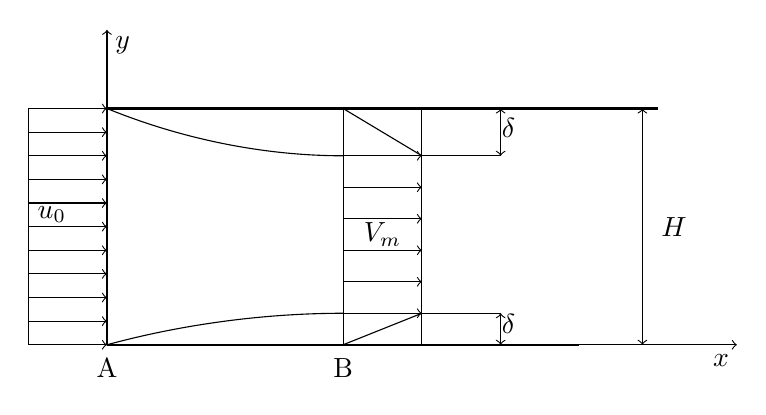
\begin{tikzpicture}

% Define coordinates for reference points A and B
\coordinate (A) at (0,0);
\coordinate (B) at (6,0);
\coordinate (C) at (0,3);
\coordinate (D) at (7,3);

% Add flow lines at inlet (uniform velocity profile at A)
\foreach \y in {0,0.3, 0.6, 0.9, 1.2, 1.5, 1.8, 2.1, 2.4, 2.7,3} {
    \draw[->] (-1,\y) -- (0,\y);
}
\foreach \y in {0.4, 0.8, 1.2, 1.6, 2, 2.4} {
    \draw[->] (3,\y) -- (4,\y);
}
% Label for u_0
\node at (-0.7, 1.65) {$u_0$};

% Draw flow lines along the channel and boundary layer growth
\foreach \x in {1.5, 3, 4.5} {
    
   
}

% Draw flow lines at B (developed profile)
\draw(3,2.4) parabola (0,3);
\draw(3,0.4) parabola (0,0);
\draw(-1,0) to (-1,3);
\draw(3,0) to (3,3);
\draw(4,0) to (4,3);
\draw(3,0) to (4,0.4);
\draw(3,3) to (4,2.4);
\draw(4,0.4) to(5,0.4);
\draw(4,2.4) -- (5,2.4);
% Boundary layer thickness labels
\draw[<->] (5,0) -- (5,0.4);
\draw[<->] (5,3) -- (5,2.4);
\node at (5.1,0.26) {$\delta$};
\node at (5.1,2.76) {$\delta$};

% Label for Vm (mean velocity)
\node at (3.5, 1.4) {$V_m$};

% Draw the height H between the plates
\draw[<->] (6.8,0) -- (6.8,3);
\node at (7.2,1.5) {$H$};

% Draw the plates
\draw[thick] (A) -- (B);
\draw[thick] (C) -- (D);

% Add x and y axes labels
\draw[->] (0,0) -- (0,4);
\node at (0.2,3.8) {$y$};

\draw[->] (-0.5,0) -- (8,0);
\node at (7.8,-0.2) {$x$};

% Labels for points A and B
\node at (0,-0.3) {A};
\node at (3,-0.3) {B};

\end{tikzpicture}

